\documentclass{article}
\usepackage{hyperref}
\usepackage{blindtext}
\usepackage{ulem}
\usepackage[T1]{fontenc}
\usepackage[utf8]{inputenc}
\usepackage{amsmath}
\usepackage{graphicx}
\usepackage{hyperref}
\usepackage{amsfonts}
\usepackage{amsmath}
\usepackage{amssymb}
\usepackage{ mathrsfs }
\usepackage{tikz}

\title{\Huge Society 2.0}
\author{Michael Simkin}
\begin{document}
	\maketitle
	\section{Introduction}
	
	The major goal of Society 2.0 is to crate a new kind of communication and perception of social reality. It works on two level - a personal level where each individual is capable to find its own group of people according to his personality, interests, location, system of beliefs (moral values) etc. As well to promote communication between members of the groups to create identity and meaning to the collective as a whole. And be capable to communicate between collectives in the same meaningful way as we communicate between people. Another major part is to make everything as customization as possible, and receive as maximum feedback from the users as possible. Each individual can create its own interface of Q\&A. For example someone wants only finger up and down, someone else a scale from 1 to 5 etc. It also promotes physical meetings over virtual ones (and virtual meeting over forum or email).\\
	
	Society 2.0 is an app that has two faces. An outer face and an inner face. From the outside it's sort of constantly evolving tamaguchi. And from the inside it's a social network. \\
	
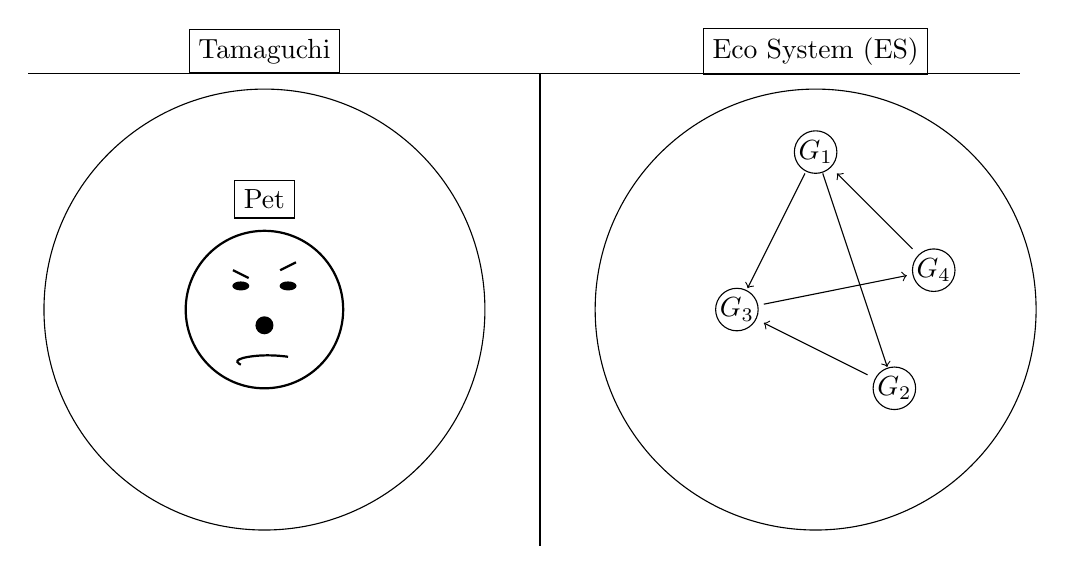
\begin{tikzpicture}


\draw (0,0)circle(2.8);
\draw (-3,3) -- (9.6,3);

\draw (3.5,3) -- (3.5,-3);

\draw (7,0)circle(2.8);

\node [draw] at (0,3.28) {Tamaguchi};
\node [draw] at (0,1.4) {Pet};
\node [draw] at (7,3.28) {Eco System (ES)};

\draw[thick] (0cm,0cm) circle(1cm);
\draw[thick] plot [smooth,tension=1.5] coordinates{(-0.3,-0.7) (-0.2,-0.6) (0.3,-0.6)};
\draw[thick] (-0.4,0.5) -- (-0.2,0.4);
\draw[thick] (0.4,0.6) -- (0.2,0.5);
\draw [thick, fill=black] (0,-0.2) circle (0.1);
\draw [rotate=90, fill=black] (0.3,0.3) ellipse (0.05 and 0.1);
\draw [rotate=90, fill=black] (0.3,-0.3) ellipse (0.05 and 0.1);

\draw (7,2)circle(0.27) node (G1) {$G_{1}$};
\draw (8,-1)circle(0.27) node (G2) {$G_{2}$};
\draw (6,0)circle(0.27) node (G3) {$G_{3}$};
\draw (8.5,0.5)circle(0.27) node (G4) {$G_{4}$};

\draw[->]
(G1) edge (G2) (G2) edge (G3) (G3) edge (G4) (G1) edge (G3) (G4) edge (G1);


\end{tikzpicture}

Where the $\{G_{i}\}$ are social groups inside the ES, the arrows indicate messages passing between the groups. The ES wants to survive and therefore it rewards for messages which bring more activity and users for the ES. Tamaguchi is also managed by the ES to be most attractive to the users. Unlike regular networks ES has special reward for making physical contacts between members of the group (any group defines its own rules but the ES reward physical interaction and not only virtual ones). This property of the app is similar to having a pet, which wants to make a walk and meet other members of its clan.  \\

To optimize communication ES has several visualization and optimization tools of the social reality. One such tool is zoom in-out from the local to the global and back. For example we can zoom on earth, and we can zoom on scientific fields of research. In the case of science we will have social map which looks more like a tree. ES is also made to optimize communication between groups. For example if Israelis have hard time to speak to Palestinians maybe they can talk with several nodes on the graph which will transform the message in more acceptable for the other guys form. Yet still the message will pass from one group to another, and it's scale independent - per each group size there would be different tools to create message and generate social consensuses. 

\section{Coherent individual}

Our knowledge about the subjectivity of other people is based only on their report about themselves, and our internal models of personality. Every time a person reports something improbable about himself we will prefer to use our models, while when it's something probable enough we shell believe him. As long as we trust the individual about self report we can summarize our knowledge of him into a long string of propositions about himself made by him or others who describe him. The string is a list of sentences about the inner world and personality of this person which someone claims to be true. \\

In order to have a group of individuals we need at least some relatively rough representation of single individual. As space of sentences is final, and only some of them describe a taken individual well, we can say a person can be represented as a list of correct sentences about this individual (or at least more correct than incorrect - we can approach it as continuous measure), which is basically equivalent to some ellipsoid in final space. \\

Coherence is prerequisite for moving to the group level. If a person can't explain or express his feelings and state of mind in any coherent way we can grasp, there is nothing we can do for him. A person could be partially coherent, for example a person can say coherent sentences about buildings but incoherent about politics. As long as a person is answering in a coherent manner to questions he's asked, we can say the person has some point of view we should take into account. At the moment a person himself is incoherent, his view will need to be reviewed and modified, yet still his opinion due to incoherence will be disqualified in any group where personal coherence is prerequisite. Hopefully more groups will require personal coherence, otherwise the group will be influenced by random incoherent forces coming from random directions - and thus the group voice will become just white noise. 

The strong coherence criteria is to have no logical faults. The least strict is not contradicting yourself inside an "official" argument. We can generate coherence score using some exams, as coherence is measurable skill. 

\section{Coherent group}

Lets assume we have a group of individuals $G_{0}$=\{$A_{i}$\}. This is not obvious but the move from being an empirical set of individuals and a set of individuals who recognize themselves as a group - is something only possible to humans using human brain i.e. there is no civilization of other primates or anything close to it. This self identification as being part of society on larger scales than several hundreds is unique to humans. This means that the parentheses around $Ai$ is very not trivial operation. But we know people are doing it anyway, this is part of human capacity to recognize oneself as being part of a group. For example I'm having hard time to convince individual to think about themselves as part of humanity. People use to think about themselves as part of a city or a country but not a species. \\

So lets assume we have group $G_{0}$ and we want to run query $Q:G_{0} \to [-1,1]$ (Q could be a question or a statement etc). But inside the group we can only run query on individual $A_{i} \in G_{0}$. So now we theoretically have an answer which is $ [-1,1]^n \ where \ n = |G_{0}|$. How do we deduce from it an answer which is comparable? Currently most of the solutions using just vote counting, but the actual question is as follows: assuming we have a group $G_{0}$ and assuming we're having query Q to generate a comparable answer of agreement or disagreement of the group with this Q. So one solution is to have agreement inside the group with function $F:[-1,1]^n \to [-1,1]$. Or we we can enforce some answer by some dictator etc. We can also ask several professional opinions or make some more complex functions to optimize the precision and quality of the result according to situation. \\

Modern democracy is also such function $F$ which tries to appeal to justice on one hand and to coherence on the other. We still have a king, but only for limited amount of time. My main question is: can't we generate coherent hive mind, which will include all the answers by many people, and still generate coherent and "just" statements, and probably capable of generating super human decisions, because many people contain more information and have more knowledge than any specific individual. 
\\
\section{Groups Types}

The alpha version of Society 2.0 is intending to implement very small amount of groups. 

\renewcommand{\labelitemii}{$\star$}

\begin{itemize}
	\item Local Group
\begin{itemize} 
	\item Neighborhood
	\item City
	\item Country
	\item Planet
\end{itemize}
	\item Skill Group 
\begin{itemize} 
	\item Sport (chess, tennis, woodcraft 3)
	\item Knowledge (programming, teaching math, scientific area)
	\item Subjective (art, discoveries, beauty)
\end{itemize}
	\item Shared interest Group
\begin{itemize} 
	\item Buy-Sell
	\item Promote project (solve problem, play music)
	\item Dating
\end{itemize}
	
\end{itemize}

\section{Social order}

In Society 2.0 special emphasis is done on complete freedom of self definition of the group, expressing this freedom in the interface of the group, and sharing experience between groups to improve a set of parameters each group defines for itself as important (and obviously to benefit the ES).\\

Each group has rules, news, goals, meetings, social status of members and communication protocols within the group and with members from other groups etc. as part of self definition of the group. Everything inside the group can be defined by the group members themselves i.e. there is no group admin or group owner unless the group is defined this way. Special tools are devised to express group agenda using queries on the group and install the results of the queries inside the group social order as part of self definition. \\

Every time a new decision is installed - each member of the group has a choice to continue to be part of the group with the new rule which he's not agrees with or to become part of another group (i.e. to leave and organize automatically a group with opposite rule or without the rule). \\

This will inherently create a balance between the group that wants to have a power of many - and a group that wants to create new agendas and evolve. This we will get a tree of groups, in the root there would be a set of rules agreed upon all "mega group" members, and a lot of sub groups of different sizes which share some parts of goals and rules. There are several good reasons to not split a group due to new decisions, as number of splits is very limited by math, and larger groups can evolve faster as they have more resources. \\

Examples of social orders: 
\begin{itemize} 
	\item Pyramid
	\item Hive mind
	\item Real democracy
	\item Leaky pyramid
	\item Aristocracy
	\item Anarchy
	\item Capitalism
	\item Military dictatorship 
	\item Communism 
	\item Feudalism
\end{itemize}

For example currently in local realms we have something between military dictatorship (i.e. enforced order) and aristocracy (a social pyramid which the people can only choose from the top). In the workplace we currently have feudalism, people usually treat the worker as available resource and usually there is a boss (the feudalistic lord). This haven't skipped the virtual realm, just the name switched to admin. For society that has an internet our social order is ill developed and still uses mainly force to enforce policies, just like the ancient Romans and Greeks from 2500 years ago, using very similar social structure. Looks like no one thought of any better idea in 2500 years - people thought of worse ideas like communism and fascism. 

\section{Standard subgroups}

In Society 2.0 each group comes with two predefined subgroups. One is a subgroup of "meta cognition group", those people are thinking about the group self definition and goals. For example many people from group of chess players will not want to think about the goals of the chess players groups. They just want to play chess (and if the group rules are too demanding to leave a feedback to the meta cognition group - please change this or that rule). \\

Another group are customizers of group rules (some of them might be programmers). This group is only implementing the decisions inside the UI of the group consensus. This is technical part of the group. For large groups which has a lot of rules, big portion of resources of the group as well as shared experience will be concerning this group. 

\section{Physical Meetings}

Physical meetings are encouraged by the tamaguchi, and meeting protocols are devised per each in-group and inter-group meetings. For example if I play chess and you play chess - the protocol of meeting will advice us to play 5 min. game. The game result is then recorded and "transaction" is registered. This kind of interaction is also promoting the ES, thus points for such behavior will come from the ES to the people and to the chess group. If I play chess and you tennis, we can still have some inter-group communication for example we can think about common solution for both sports, and learn from each other thus devising some new scoring strategy or cooperation for promoting the sports (or invent chess-tennis a new sport like chess-boxing). \\

Every person can also agree to be sent to a mission by the group. For example a hardcore chess player would like to play in a chess club, but we can register transaction without the need of a chess club. We can play 2hr online or in some park, as well as we can promote taking chess lessons instead of just playing a game, and keep track of better chess teachers and not only chess players. As teaching chess is commodity inside the chess players community, we can recognize the best chess teachers and make them teach other teachers how to teach chess etc. \\

Some more complex inter-group meeting protocols could be devised. For example maybe it's a bad idea to let Christians to speak with Satanists. Some rules can be devised to promote separation of groups, yet still make sure the group graph is connected and most important news are spreading among all groups. Also messages can be sent from one group to another through proxies. It's important that they will acknowledge the mere fact of existence of each other. \\

\section{Eco System}

EcoSystem is a class which is not concerned with specific goals of individuals. It's a representative of an app, that wants to survive. For this purpose (except of an ES developers group), it uses points, badges, currency etc. The slogan here "if the Eco System is happy everyone are happy". As all the groups and activity and all the good features are part of the ES, the survival of the ES is most crucial for the whole user group. Because we try to share and learn from experience of each other, promoting the ES is integral part of being user of Society 2.0. \\

The happiness of ES can be expressed in simple formula to star with: 
\begin{align*}
Happ(ES) = |G_{users}| + Act(G_{users}) + Phys(G_{users}) + \frac{\partial |G_{users}|}{\partial t} 
\end{align*}

\section{Tamaguchi}

ES is also using tamaguchi, a front face of the app to promote survival. The tamaguchi is representing the community needs and satisfaction with the user activity. The basic assumption is that the user likes his tamaguchi to be happy. When two people meet, their tamaguchis are exchanging knowledge of reality and they are happy. The app is promoting phone to phone transactions.\\ 

The tamaguchi is developed by special developing group - the tamaguchi skill group. Every new tamaguchi version is first tested on a subset of users, and scored for H(ES) for those users. Tamaguchi developers are scored by the ES very highly as they are the front face of the app, and on them depends the future of the ES. This group is consisting of visual designers and programmers who work together to make the tamaguchi as cute as possible or whatever makes the ES happy. 

\section{Versioning \& source}

Society2.0 believes in freedom of information and that open source will cooperate with other open source while closed source will die out in larger scales. The current state of law and economics are artificially promoting big companies and close source, when alternative solutions will be found by the app - the freedom of information and its increasingly developing paste will overcome the shortcomings of current law and economy systems. It has no owner no master, it's a living creature which spreads by interaction between people. \\

A person who wants to upgrade the ES to a new version, will need to trust his fellow who gives him the new version. This is not to say there are no groups which are developing the ES and compete among themselves. There is a version tree which is hardcoded inside the first version to allow back compatibility. New branches are promoted by the ES as they could bring more users. At the moment too much branching is limiting the growth of ES it will alert the developers to cooperate instead of compete, in order to close the gaps between different versions. 

\section{Zoom out}

One of the major features of Society 2.0 is the ability to Zoom in-out from your local group and see the "big picture". To realize you're not only part of a group but also part of an Eco System which has a lot of different groups and tries to make everyone live in peace with everyone else using communication. This will be presented to every user visually. \\

When you enter the ES you see this happening. All the groups, people, activity, ideas. You have a sense of entering something "living", even before you dive in and start to join groups and develop personal coherence skills. \\

As the ES is trying to promote communication and transaction and collective cooperation and self definition one should left to only notice that this is the only thing there is in a social realm. If all people will agree on something this something will become a reality. \\



\end{document}









